\section{Introduction and Notation}\label{sec:intro}

For the reader that has never come across permutations before, they can be described simply as a rearrangement of some objects. This book will focus on \textit{permutation cycles}, which are permutations of whole numbers. We shall consider sets of whole numbers that start at \(1\) and include every whole number up to a given value, such as \(\{1, 2, 3, 4, 5, 6, 7, 8\}\) like on the front cover.

This book will do its best to avoid assuming too much prerequisite knowledge on the readers' behalf, but an understanding of basic set theory, algebra, and group theory will be helpful. As this is an introductory guide, this is intended for individuals who do not yet grasp permutations. Readers with an understanding of permutations will find this book slow.

It is important for the reader to realise that notation in much of Mathematics is not fixed -- that is, there are many ways of writing the same thing. There are general conventions, but every author has the freedom to write things in a way that makes the most sense to them, and the notation for permutations is certainly vast because of this. Not only are there multiple ways of writing the same permutation, there are also many ways of writing compositions of permutations, and also compact ways of describing certain permutation structures. This first chapter will present the most popular notations, including an abundance of examples to gain an understanding of how they work.

There are also exercises throughout. They do not have to be completed in order to understand the following contents of the book. However, it is strongly advised that they are at least attempted, since they offer an opportunity to build familiarity with permutations.

%%%%%%%%%%%%%%%%%%%%%%%%%%%%%%%%%%%%%%%%%%
%%%%%%%%%%%%%%%%%%%%%%%%%%%%%%%%%%%%%%%%%%

\subsection{Preliminaries: maps and sets}

This section introduces the notions of sets, maps, and groups for a clarification on notation, and also to make this text accessible to readers without much formal background in Mathematics. These notions will be covered quickly though, and a reader with the intention to understand these deeper is directed to relevant textbooks.

A \textit{set} is a collection of elements, typically numbers or letters, written between the braces \(\{\,\,\}\). We may refer to a set of elements -- say the set containing \(a\), \(b\), and \(c\), written \(\{a, b, c\}\) -- by a single letter, say \(S\). In this case, we write that \(S = \{a, b, c\}\). Repeated elements are typically avoided in sets, so that the set \(\{a, b, b, c, a, d\}\) is written simply as \(\{a, b, c, d\}\). The order in which the elements are listed does not matter in a set, so \(\{a, b, c, d\}\) and \(\{d, a, c, b\}\) are regarded as the same set, for example.

Given some set \(A\), we will write \(a \in A\) for \(a\) is an element of \(A\), and \(A\backslash\{a\}\) for the set \(A\) without the element \(a\). Given another set \(B\), if every \(b \in B\) is also in \(A\), then \(B\) is a \textit{subset} of \(A\) which is written \(B \subseteq A\). If \(B \subseteq A\) and it is known that there are elements in \(A\) that are not in \(B\), we will write this as \(B \subset A\) and call \(B\) a \textit{proper subset} of \(A\). If \(B\) and \(A\) have identical elements, then they are equal as sets and we write \(A = B\). The set \(A\) with all of the elements of \(B\) removed from \(A\) is written \(A\backslash B\). The \textit{cardinality} of \(A\) is the number of elements in \(A\), and is written \(|A|\). More on set theory and the notations used here can be found in Halmos' \textit{Naive Set Theory} \cite{Halmos}.

A \textit{map} \(f\) from a set \(A\) to a set \(B\), written \(f \colon A \to B\), is an assignment to each \(a \in A\) exactly one element \(b \in B\), commonly written \(f(a) \in B\) and called the \textit{image of \(a\) under \(f\)}, or simply as the \textit{image of \(a\)} if the map \(f\) is understood. It is common to call \(A\) the \textit{domain} and \(B\) the \textit{range} (or \textit{codomain}). We write \(a\) maps to \(f(a)\) as \(a \mapsto f(a)\), or if \(b = f(a)\) then we can write \(a \xmapsto{f} b\). If \(f\) is clear, then we may write just \(a \mapsto b\). Figure~\ref{fig:bijmap} illustrates this with the sets \(A = \{1, 2, 3\}\) and \(B = \{2, 3, 4\}\), with the map \(f\) defined as
\[
1 \xmapsto{f} 3, \hspace{20pt} 2 \xmapsto{f} 2, \hspace{20pt} 3 \xmapsto{f} 4,
\]
or, equivalently,
\[
f(1) = 3, \hspace{20pt} f(2) = 2, \hspace{20pt} f(3) = 4.
\]
For those new to maps, a map is a generalisation of a function (though some authors may call maps functions) since a function is just a map from subsets of \(\R\) to subsets of \(\R\). We write \(\R\) for the set of \textit{real numbers}, which includes all positive and negative fractions and decimals, including numbers like \(\pi\).

Note that in the example above \(A\) is not equal to \(B\), written \(A \neq B\), since \(A\) contains \(1\) but not \(4\), and \(B\) contains \(4\) but not \(1\). It's also important to notice that even though \(A\) and \(B\) share two of the same numbers, this has no relevance to how \(f\) is defined. Although \(A \neq B\), we have that \(|A| = 3\) and \(|B| = 3\), so that \(|A| = |B|\).

\begin{figure}[h]
    \centering
    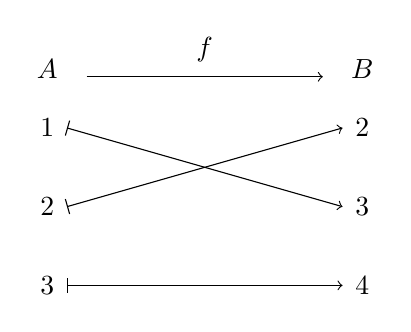
\begin{tikzpicture}
        \node at (-2, -1) {\(3\)}; \node at (-2, 0) {\(2\)}; \node at (-2, 1) {\(1\)}; \node at (-2, 1.75) {\(A\)};
        \node at (2, -1) {\(4\)}; \node at (2, 0) {\(3\)}; \node at (2, 1) {\(2\)}; \node at (2, 1.75) {\(B\)};

        \draw[->] (-1.5, 1.65) -- (1.5, 1.65); \node at (0, 2) {\(f\)};
        \draw[|->] (-1.75, -1) -- (1.75, -1); \draw[|->] (-1.75, 0) -- (1.75, 1); \draw[|->] (-1.75, 1) -- (1.75, 0);
    \end{tikzpicture}
    \caption{The diagram of the map \(f \colon A \to B\).}
    \label{fig:bijmap}
\end{figure}

\begin{definition}[(Bijective map)]
    Let $f \colon A \to B$ be a map between two sets. Then $f$ is \textit{injective} (also known as \textit{one-to-one}) if the images $f(a) \in B$ are distinct for each $a \in A$. We say that $f$ is \textit{surjective} (also known as \textit{onto}) if every $b \in B$ is the image of at least one element $a \in A$. If $f$ is both injective and surjective, then $f$ is said to be \textit{bijective} and $f$ is a \textit{bijection} between $A$ and $B$.
\end{definition}

If the sets $A$ and $B$ are finite and there is a bijection $f$ between them, then the cardinality of $A$ is necessarily equal to the cardinality  of $B$. The function $f$ defined in Figure~\ref{fig:bijmap} has this bijective property: each image is unique, and every element in $B$ is the image of some element in $A$.

Maps only give information about the relationship between sets, but doesn't give the sets themselves a structure. A \textit{group} is a set of elements that \textit{does} have some kind of structure as there is a relationship between every one of the elements in a group. In particular, the set $G$ is a group if there is a binary operation (an operation taking two inputs), commonly multiplication, so that two elements of $G$ can be combined to give another element of $G$. For the full definition of a group, see Section~\ref{subsec:groups}. There is no shortage of introductory textbooks that discuss groups.

%%%%%%%%%%%%%%%%%%%%%%%%%%%%%%%%%%%%%%%%%%
%%%%%%%%%%%%%%%%%%%%%%%%%%%%%%%%%%%%%%%%%%

\subsection{Permutations and their diagrams}

We can now start to define permutations. Let $\Omega_{n}$ denote the set of whole numbers from $1$ to $n$ for some whole number $n$. For example, the set $A = \{1, 2, 3\}$ above would now be written $\Omega_{3} = \{1, 2, 3\}$. The symbol $\Omega$ is the capital Greek letter omega.

\begin{definition}[(Permutation)]
    A \textit{permutation} $\sigma \colon \Omega_{n} \to \Omega_{n}$ is a bijective map from the set $\Omega_{n}$ to itself. We can say \textit{$\sigma$ is a permutation on $\Omega_{n}$} to mean that $\sigma$ is a map $\sigma \colon \Omega_{n} \to \Omega_{n}$.
\end{definition}

From the definition, a permutation is just a map that takes a number in $\Omega_{n}$ and sends it to another (possibly the same) number in $\Omega_{n}$. For this reason, we can write a permutation in the same way that one might define a map, just like how $f$ was defined above. However, there are many ways that this permutation can be written, and we will demonstrate a number of them with a specific example.

\begin{example}
    Let $\sigma$ be a permutation on $\Omega_{5}$ defined by
    \[
    \sigma(1) = 1, \hspace{20pt} \sigma(2) = 3, \hspace{20pt} \sigma(3) = 4, \hspace{20pt} \sigma(4) = 2, \hspace{20pt} \sigma(5) = 5.
    \]
    This uses the notation of maps defined as above, but it is not the most common. A more common notation is the \textit{two-line} representation where the image of an element is written beneath it. For the current example, we could write $\sigma$ as
    \[
    \begin{pmatrix}
        1 & 2 & 3 & 4 & 5 \\
        1 & 3 & 4 & 2 & 5 \\
    \end{pmatrix}.
    \]
    This is read from top to bottom, so that $1 \xmapsto{\sigma} 1$ by the first column, with $2 \xmapsto{\sigma} 3$ by the second column, and so on (remember $a \xmapsto{\sigma} b$ and $\sigma(a) = b$ are interchangeable). The precise order of the columns does not matter, only that the correct images come under each element. Thus, the following ways of writing $\sigma$ are all equivalent:
    \[
    \begin{pmatrix}
        \textcolor{green!50!black}{1} & \textcolor{blue!50!black}{2} & \textcolor{red!50!black}{3} & \textcolor{yellow!50!black}{4} & 5 \\
        \textcolor{green!50!black}{1} & \textcolor{blue!50!black}{3} & \textcolor{red!50!black}{4} & \textcolor{yellow!50!black}{2} & 5 \\
    \end{pmatrix} = \begin{pmatrix}
        5 & \textcolor{yellow!50!black}{4} & \textcolor{red!50!black}{3} & \textcolor{blue!50!black}{2} & \textcolor{green!50!black}{1} \\
        5 & \textcolor{yellow!50!black}{2} & \textcolor{red!50!black}{4} & \textcolor{blue!50!black}{3} & \textcolor{green!50!black}{1} \\
    \end{pmatrix} = \begin{pmatrix}
        \textcolor{green!50!black}{1} & 5 & \textcolor{blue!50!black}{2} & \textcolor{red!50!black}{3} & \textcolor{yellow!50!black}{4} \\
        \textcolor{green!50!black}{1} & 5 & \textcolor{blue!50!black}{3} & \textcolor{red!50!black}{4} & \textcolor{yellow!50!black}{2} \\
    \end{pmatrix} = \begin{pmatrix}
        \textcolor{blue!50!black}{2} & \textcolor{red!50!black}{3} & \textcolor{yellow!50!black}{4} & \textcolor{green!50!black}{1} & 5 \\
        \textcolor{blue!50!black}{3} & \textcolor{red!50!black}{4} & \textcolor{yellow!50!black}{2} & \textcolor{green!50!black}{1} & 5 \\
    \end{pmatrix}.
    \]
    The general way of writing $\sigma : \Omega_{5} \to \Omega_{5}$ in this form is
    \[
    \sigma = \begin{pmatrix}
        1         & 2         & 3         & 4         & 5 \\
        \sigma(1) & \sigma(2) & \sigma(3) & \sigma(4) & \sigma(5) \\
    \end{pmatrix}.
    \]

    Some authors have been known to fix the top row so that it reads $1$, $2$, $\ldots$, $n$ and then write just the bottom row, as the top row is taken to be understood from context. In this way, we would write $\sigma$ as
    \[
    (1 \q 3 \q 4 \q 2 \q 5)
    \]
    which we shall call \textit{reduced two-line form}. For this notation, if a number is in the $i^{\,\text{th}}$ position, then it is the image of $i \in \Omega_{n}$ under $\sigma$. For example, the $2$ above is in the fourth position, so we understand this as $4 \xmapsto{\sigma} 2$. The general way of writing $\sigma : \Omega_{5} \to \Omega_{5}$ in this form is
    \[
    \sigma = \big(\sigma(1) \q \sigma(2) \q \sigma(3) \q \sigma(4) \q \sigma(5)\big).
    \]
    This way of writing permutations can cause confusion with the following one-line cycle notation, so we will avoid it as much as possible. Note also that this form is the least tangible since the representation
    \[
    \big(\sigma(1) \q \sigma(2) \q \sigma(3) \q \ldots \q \sigma(n)\big)
    \]
    is unique for the permutation $\sigma$ unlike the other representations, as the order in which the elements appear is fixed. For some authors, the fact that this representation is unique is useful when determining exactly how many permutations there are for each set $\Omega_{n}$ (see Section~$*$).

    The most common way to write permutations is the one-line \textit{cycle notation}. In this form, the permutation $\sigma$ would be written
    \[
    \sigma = (1)(2 \q 3 \q 4)(5).
    \]
    The insides of the brackets (called a cycle) are read from left-to-right, with the rightmost element in the cycle `cycling back' to the first element. That is, if we were to read $(2 \q 3 \q 4)$ as a cycle permutation, this indicates that $2$ maps to $3$, that $3$ maps to $4$, and that $4$ maps back round to $2$. Similarly to the two-line notation, the only important positioning is what comes directly before and directly after each element, so the following are all equivalent:
    \[
    (2 \q 3 \q 4) = (4 \q 2 \q 3) = (3 \q 4 \q 2).
    \]
    All three of the above indicate that $2$ maps to $3$, that $3$ maps to $4$, and that $4$ maps to $2$, irrespective of whichever number comes first in the brackets. One can see why they are appropriately named \textit{cycles}. In the permutation $\sigma$, the solitary $(1)$ and $(5)$ mean that $1$ maps to itself and that $5$ maps to itself. These are referred to as \textit{fixed points}, and are typically omitted from the written permutation as unwritten elements are understood to be fixed points. In this case, we can say that $\sigma$ \textit{fixes} both $1$ and $5$, and that both $(1)$ and $(5)$ are \textit{trivial cycles}. That means that we can write $\sigma$ as
    \[
    \sigma = (1)(2 \q 3 \q 4)(5) = (2 \q 3 \q 4).
    \]
    This is certainly more compact than the two-line form. These can also be represented by diagrams, much like Figure~\ref{fig:bijmap}. Figure~\ref{fig:sigma} show just two ways of drawing the permutation $\sigma$: the left is the analogue of the two-line form, and the right is the analogue of the one-line cycle form. We will call a drawing that is the analogue of the one-line form of a permutation its \textit{diagrammatic form}.

    \begin{figure}[ht]
        \centering
        \begin{tikzpicture}[scale=1]
            \begin{scope}[shift={(0, 0)}]
                \foreach \x in {1, 2, 3, 4, 5}
                    \node at (1.5*\x - 4.5, 1) {$\x$};
                \foreach \x in {1, 2, 3, 4, 5}
                    \node at (1.5*\x - 4.5, -1) {$\x$};

                \draw[|->] (-3, 0.75) -- (-3, -0.75);
                \draw[|->] (-1.5+.2, 1-0.2666) -- (-0.2, -1+0.2666);
                \draw[|->] (0.2, 1-0.2666) -- (1.5-0.2, -1+0.2666);
                \draw[|->] (1.25, 0.875) -- (-1.25, -0.875);
                \draw[|->] (3, 0.75) -- (3, -0.75);
            \end{scope}
            \begin{scope}[shift={(8.5, 0)}]
                \node at (-2.3094, 1) {$1$}; \node at (-1.1547, -1) {$2$}; \node at (0, 1) {$3$}; \node at (1.1547, -1) {$4$}; \node at (2.3094, 1) {$5$};

                \draw[|->] (1.1547-0.25, -1) -- (-1.1547+0.25, -1); \draw[|->] (-1.1547+0.1443, -0.75) -- (-0.1443, 0.75); \draw[|->] (0.1443, 0.75) -- (1.1547-0.1443, -0.75);
                \draw[|->] (-2.3094, 0.75) arc (-180:90:0.25); \draw[|->] (2.3094, 0.75) arc (0:-270:0.25);
            \end{scope}
        \end{tikzpicture}
        \caption{Two ways of drawing $\sigma$.}
        \label{fig:sigma}
    \end{figure}
\end{example}

To generalise the above example, we define two representations of permutations.\newpage

\begin{definition}[(Two-line form)]
    Given a permutation $\sigma \colon \Omega_{n} \to \Omega_{n}$, the \textit{two-line form} of $\sigma$ is
    \[
    \begin{pmatrix}
        1         & 2         & 3         & \cdots & n \\
        \sigma(1) & \sigma(2) & \sigma(3) & \cdots & \sigma(n) \\
    \end{pmatrix}
    \]
    where $\sigma(i)$ is the image of element $i$ under the permutation $\sigma$, in mapping notation. Observe that the number of columns is precisely the number of elements being mapped. The \textit{reduced two-line form} of $\sigma$ is
    \[
    \big(\sigma(1) \q \sigma(2) \q \sigma(3) \q \cdots \q \sigma(n)\big).
    \]
\end{definition}

We will use these representations less often than the following one-line form, but it is important to note that this notation is used by a variety of authors.

\begin{definition}[(One-line form)]
    Given a permutation $\sigma \colon \Omega_{n} \to \Omega_{n}$, the \textit{one-line form} of $\sigma$ is the (possibly multiple distinct) cycle(s) of elements in $\Omega_{n}$, as described in the above exercise. This is also called \textit{cycle notation}.
\end{definition}

Some authors use commas in the cycles to separate the elements, so some authors would write $(2, 3, 4)$ instead of $(2 \q 3 \q 4)$, for example. This will be avoided in this book, as the use of commas this way could cause confusion with the \textit{vector} consisting of the same elements, and with notation that will be introduced in Section~$*$.

Even though there may be multiple cycles of elements in a \textit{single} permutation, no element will repeat in any of the cycles by the bijective property of permutations (see the following exercise), so the cycles are all \textit{disjoint}. The focus of the next section is to discover how to work with permutations when there are multiple cycles with shared elements.

\begin{example}
    Some non-examples of permutations in two-line form would be the following:
    \[
    \sigma_{1} = \begin{pmatrix}
        1 & 2 & 3 & 4 & 5 \\
        2 & 2 & 3 & 5 & 4 \\
    \end{pmatrix}, \hspace{20pt} \sigma_{2} = \begin{pmatrix}
        5 & 4 & 3 & 4 & 5 \\
        1 & 2 & 3 & 4 & 5 \\
    \end{pmatrix}, \hspace{20pt} \sigma_{3} = \begin{pmatrix}
        5 & 4 & 3 & 2 & 1 \\
        1 & 2 & 3 & 6 & 5 \\
    \end{pmatrix}.
    \]
    The first `permutation' $\sigma_{1}$ is not really a permutation because both $1$ and $2$ map to $2$, which violates the injective property of permutations (since every image has to be unique), and also $1$ not the image of any permutation (so $\sigma_{1}$ is not surjective either). The second `permutation' $\sigma_{2}$ is not really a permutation because $5$ maps to both $1$ and $5$, and also $4$ maps to both $2$ and $4$. While $\sigma_{2}$ is surjective with distinct images, this is not a well defined map because every element should have \textit{exactly one} image. Finally, the `permutation' $\sigma_{3}$ is not really a permutation because there are more elements than there are columns. Even though every image is distinct, the $6$ in the bottom row would indicate that the permutation is a map $\sigma_{3} \colon \Omega_{6} \to \Omega_{6}$, but the map has not been defined for $6$ since $6$ does not appear on the top row.

    An important thing to check with two-line permutations is that every element appears exactly once in the top row, exactly once in the bottom row, and there are the same number of distinct elements as there are columns. To be more precise, there are $n$ columns in the permutation if and only if every element from $1$ to $n$ (that is, every element in $\Omega_{n}$) appears exactly once in the top row and exactly once in the bottom row. All three of the above `permutations' fail this, which is why they are not well defined permutations.

    Two non-examples of permutations in one-line form would be the following:
    \[
    \sigma_{1} = (1 \q 3 \q 2 \q 4 \q 3 \q 5), \hspace{20pt} \sigma_{2} = (1)(2)(3 \q 4 \q 3).
    \]
    The first `permutation' $\sigma_{1}$ is not really a permutation because both $1$ and $4$ map to $3$ so $\sigma_{1}$ is not injective, and $3$ maps to both $2$ and $5$ so $\sigma_{1}$ is not a well defined map. The second `permutation' $\sigma_{2}$ is not really a permutation because the final cycle indicates that $3$ maps to $4$, then $4$ maps to $3$, \textit{and then $3$ maps back round to $3$}. That is, in this cycle $3$ maps to both $4$ and $3$, so that this is not a well defined map. Also, since both $3$ and $4$ map to $3$, it is not injective either.

    An important thing to check with one-line permutations is that every element appears exactly once in each cycle. Both of the permutations above fail this, which is why they are not well defined permutations.
\end{example}

%%%%%%%%%%%%%%%%%%%%%%%%%%%%%%%%%%%%%%%%%%
%%%%%%%%%%%%%%%%%%%%%%%%%%%%%%%%%%%%%%%%%%

\subsection{Permutation composition: right-to-left}

By the way that permutations have been defined, it makes sense to consider them as maps. In the general representations of a permutation, we even use the notation of a map in the very definition! From this perspective, many authors define the product of two permutations to be the composition of the permutations viewed as maps. Given two permutations $\sigma$ and $\gamma$, this would mean that $\gamma\sigma$ is short for $\gamma \circ \sigma$ (with the $\circ$ symbol the typical notation for composition of maps and functions), where the permutation $\sigma$ is applied first, followed by $\gamma$.

\begin{example}\label{eg:siggam}
    Let $\sigma = (1 \q 2 \q 3 \q 4)$ and $\gamma = (1 \q 3 \q 2)$ be two permutations on $\Omega_{4}$ in one-line cycle form. Note that we have written $\gamma$ as $(1 \q 3 \q 2)$ instead of the slightly longer $(1 \q 3 \q 2)(4)$ because we know that if an element has not been written, then it is a fixed point. In two-line form, we could have written $\sigma$ and $\gamma$ respectively as
    \[
    \sigma = \begin{pmatrix}
        1 & 2 & 3 & 4 \\
        2 & 3 & 4 & 1 \\
    \end{pmatrix} \textand \gamma = \begin{pmatrix}
        1 & 2 & 3 & 4 \\
        3 & 1 & 2 & 4 \\
    \end{pmatrix},
    \]
    and if we wanted to define them as maps we could have written
    \[
    \begin{array}{cccc}
        \sigma(1) = 2, \hspace{20pt} & \sigma(2) = 3, \hspace{20pt} & \sigma(3) = 4, \hspace{20pt} & \sigma(4) = 1, \\[8pt]
        \gamma(1) = 3, \hspace{20pt} & \gamma(2) = 1, \hspace{20pt} & \gamma(3) = 2, \hspace{20pt} & \gamma(4) = 4. \\
    \end{array}
    \]
    Consider what might happen if we apply the composition $\gamma\circ\sigma$ to the element $1$. Applying $\sigma$, we have $\sigma(1) = 2$, and then we apply $\gamma$ to the result to get $\gamma(2) = 1$. This means that the permutation $\gamma\sigma$ maps $1$ to itself (remember, if we think about these as maps, this is $\gamma \circ \sigma$ which is $\sigma$ first and then $\gamma$). This can also be written a few different ways in the notation of maps, some of which are
    \[
    \gamma\sigma(1) = 1, \hspace{20pt} (\gamma \circ \sigma)(1) = 1, \textand \gamma\big(\sigma(1)\big) = 1.
    \]
    The latter two are the two most common notations to denote compositions of maps, but we will use the former the most. They are all equivalent though since they are all different ways of representing the same operation, so
    \[
    \gamma\sigma(1) = (\gamma \circ \sigma)(1) = \gamma\big(\sigma(1)\big).
    \]
    Now consider what happens if we apply $\gamma$ first, and then $\sigma$. We have $\gamma(1) = 3$ and then $\sigma(3) = 4$, so that (using all three notations) we have
    \[
    \sigma\gamma(1) = 4, \hspace{20pt} (\sigma \circ \gamma)(1) = 4, \textand \sigma\big(\gamma(1)\big) = 4.
    \]
    This example shows that permutations are generally not \textit{commutative} -- that is, the order in which the permutations are applied matters.

    Now, suppose we want to find $\gamma\sigma$ (which is $\sigma$ first, and then $\gamma$) for all values in $\Omega_{4}$. We will do this in four ways: using the definition of the permutations as maps, using the two-line representation, using a suitable diagram, and then using one-line form.

    \ulsc{Maps notation:} We already know that $\gamma\sigma(1) = 1$. Then
    \[
    \gamma\sigma(2) = \gamma\big(\sigma(2)\big) = \gamma(3) = 2
    \]
    since $\sigma(2) = 3$ by how we defined $\sigma$, so $\gamma\sigma(2) = 2$ and $\gamma\sigma$ fixes $2$ as well as $1$. Similarly,
    \[
    \gamma\sigma(3) = \gamma\big(\sigma(3)\big) = \gamma(4) = 4 \textand \gamma\sigma(4) = \gamma\big(\sigma(4)\big) = \gamma(1) = 3
    \]
    since $\sigma(3) = 4$ and $\sigma(4) = 1$ by how we defined $\sigma$, so that $\gamma\sigma(3) = 4$ and $\gamma\sigma(4) = 3$. To summarise these, we have
    \[
    \gamma\sigma(1) = 1, \hspace{20pt} \gamma\sigma(2) = 2, \hspace{20pt} \gamma\sigma(3) = 4, \hspace{20pt} \gamma\sigma(4) = 3,
    \]
    in the notation of maps. This can be written in two-line form as
    \[
    \gamma\sigma = \begin{pmatrix}
        1 & 2 & 3 & 4 \\
        1 & 2 & 4 & 3 \\
    \end{pmatrix},
    \]
    and in one-line form as $(1)(2)(3 \q 4) = (3 \q 4)$ since $1$ and $2$ are fixed points.

    \ulsc{Two-line form:} Recall that $\sigma$ and $\gamma$ are defined in two-line form as
    \[
    \sigma = \begin{pmatrix}
        1 & 2 & 3 & 4 \\
        2 & 3 & 4 & 1 \\
    \end{pmatrix} \textand \gamma = \begin{pmatrix}
        1 & 2 & 3 & 4 \\
        3 & 1 & 2 & 4 \\
    \end{pmatrix}.
    \]
    We can write the composition $\gamma\sigma$ as
    \[
    \gamma\sigma = \begin{pmatrix}
        1 & 2 & 3 & 4 \\
        3 & 1 & 2 & 4 \\
    \end{pmatrix}\begin{pmatrix}
        1 & 2 & 3 & 4 \\
        2 & 3 & 4 & 1 \\
    \end{pmatrix}
    \]
    which \textit{is read right-to-left}, as in the right permutation is read first, and then the left permutation. To find the image of $1$ under $\gamma\sigma$, we see that $1 \xmapsto{\sigma} 2$ in the right permutation, and then $2 \xmapsto{\gamma} 1$ in the left permutation. The total result is that $1 \xmapsto{\gamma\sigma} 1$. To highlight which columns we look at, the columns have been coloured in the following permutations (the image of $1$ corresponds to the green columns):
    \[
    \gamma\sigma = \begin{pmatrix}
        \textcolor{yellow!50!black}{1} & \textcolor{green!50!black}{2} & \textcolor{blue!50!black}{3} & \textcolor{red!50!black}{4} \\
        \textcolor{yellow!50!black}{3} & \textcolor{green!50!black}{1} & \textcolor{blue!50!black}{2} & \textcolor{red!50!black}{4} \\
    \end{pmatrix}\begin{pmatrix}
        \textcolor{green!50!black}{1} & \textcolor{blue!50!black}{2} & \textcolor{red!50!black}{3} & \textcolor{yellow!50!black}{4} \\
        \textcolor{green!50!black}{2} & \textcolor{blue!50!black}{3} & \textcolor{red!50!black}{4} & \textcolor{yellow!50!black}{1} \\
    \end{pmatrix}.
    \]
    The image of $2$ under $\gamma\sigma$ corresponds to the blue columns, and we see that $2 \xmapsto{\sigma} 3$ in the right permutation, and then $3 \xmapsto{\gamma} 2$ in the left permutation, so the total result is that $2 \xmapsto{\gamma\sigma} 2$. The image of $3$ under $\gamma\sigma$ corresponds to the red columns, and we see that $3 \xmapsto{\sigma} 4$ in the right permutation, and then $4 \xmapsto{\gamma} 4$ in the left permutation, so the total result is that $3 \xmapsto{\gamma\sigma} 4$. The image of $4$ under $\gamma\sigma$ corresponds to the yellow columns, and we see that $4 \xmapsto{\sigma} 1$ in the right permutation, and then $1 \xmapsto{\gamma} 3$ in the left permutation, so the total result is that $4 \xmapsto{\gamma\sigma} 3$. Thus, in two-line form, we have that
    \[
    \gamma\sigma = \begin{pmatrix}
        \textcolor{yellow!50!black}{1} & \textcolor{green!50!black}{2} & \textcolor{blue!50!black}{3} & \textcolor{red!50!black}{4} \\
        \textcolor{yellow!50!black}{3} & \textcolor{green!50!black}{1} & \textcolor{blue!50!black}{2} & \textcolor{red!50!black}{4} \\
    \end{pmatrix}\begin{pmatrix}
        \textcolor{green!50!black}{1} & \textcolor{blue!50!black}{2} & \textcolor{red!50!black}{3} & \textcolor{yellow!50!black}{4} \\
        \textcolor{green!50!black}{2} & \textcolor{blue!50!black}{3} & \textcolor{red!50!black}{4} & \textcolor{yellow!50!black}{1} \\
    \end{pmatrix} = \begin{pmatrix}
        \textcolor{green!50!black}{1} & \textcolor{blue!50!black}{2} & \textcolor{red!50!black}{3} & \textcolor{yellow!50!black}{4} \\
        \textcolor{green!50!black}{1} & \textcolor{blue!50!black}{2} & \textcolor{red!50!black}{4} & \textcolor{yellow!50!black}{3} \\
    \end{pmatrix}.
    \]
    This agrees with what we found in the preceding method.

    \ulsc{Diagrams:} To find the permutation $\gamma\sigma$ diagrammatically, we will draw the diagrams similarly to the drawing of $f$ in Figure~\ref{fig:bijmap}. The diagrams of the permutations are the content of Figure~\ref{fig:gammasigma}.

    \begin{figure}[h]
        \centering
        \begin{tikzpicture}[scale=1]
            \begin{scope}[shift={(0, 0)}]
                \foreach \x in {1, 2, 3, 4}
                    \node at (-2, -\x + 4) {$\x$};
                \foreach \x in {1, 2, 3, 4}
                    \node at (2, -\x + 4) {$\x$};

                \node at (-2, 3.75) {$\Omega_{4}$}; \node at (2, 3.75) {$\Omega_{4}$}; \draw[<-] (-1.5, 3.75) -- (1.5, 3.75); \node at (0, 4) {$\gamma$};

                \draw[|->] (1.75, 2.875) -- (-1.75, 1.125);   %  1 -- 3
                \draw[|->] (1.75, 2.0625) -- (-1.75, 2.9375); %  2 -- 1
                \draw[|->] (1.75, 1.0625) -- (-1.75, 1.9375); %  3 -- 2
                \draw[|->] (1.75, 0) -- (-1.75, 0);           %  4 -- 4
            \end{scope}
            \begin{scope}[shift={(8.5, 0)}]

                \foreach \x in {1, 2, 3, 4}
                    \node at (-2, -\x + 4) {$\x$};
                \foreach \x in {1, 2, 3, 4}
                    \node at (2, -\x + 4) {$\x$};

                \node at (-2, 3.75) {$\Omega_{4}$}; \node at (2, 3.75) {$\Omega_{4}$}; \draw[<-] (-1.5, 3.75) -- (1.5, 3.75); \node at (0, 4) {$\sigma$};

                \draw[|->] (1.75, 2.9375) -- (-1.75, 2.0625); %  1 -- 2
                \draw[|->] (1.75, 1.9375) -- (-1.75, 1.0625); %  2 -- 3
                \draw[|->] (1.75, 0.9375) -- (-1.75, 0.0625); %  3 -- 4
                \draw[|->] (1.75, 0.1875) -- (-1.75, 2.8125); %  4 -- 1
            \end{scope}
        \end{tikzpicture}
        \caption{The diagrams of $\gamma$ (left) and $\sigma$ (right).}
        \label{fig:gammasigma}
    \end{figure}

    Notice that these have been drawn \textit{right-to-left} to reflect how we view the permutations. The same colours for each permutation shall be used as in the preceding method to draw the diagram of $\gamma\sigma$.\newpage

    \begin{figure}[ht]
        \centering
        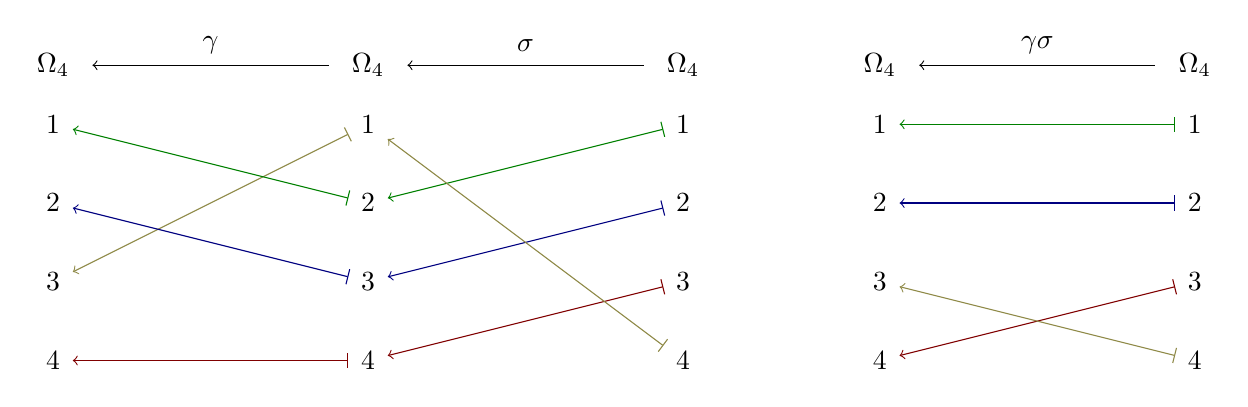
\begin{tikzpicture}[scale=1]
            \begin{scope}[shift={(0, 0)}]
                \foreach \x in {1, 2, 3, 4}
                    \node at (-4, -\x + 4) {$\x$};
                \foreach \x in {1, 2, 3, 4}
                    \node at (0, -\x + 4) {$\x$};
                \foreach \x in {1, 2, 3, 4}
                    \node at (4, -\x + 4) {$\x$};

                \node at (-4, 3.75) {$\Omega_{4}$}; \node at (0, 3.75) {$\Omega_{4}$}; \node at (4, 3.75) {$\Omega_{4}$};
                \draw[<-] (-3.5, 3.75) -- (-0.5, 3.75); \node at (-2, 4) {$\gamma$}; \draw[<-] (0.5, 3.75) -- (3.5, 3.75); \node at (2, 4) {$\sigma$};

                \draw[|->, yellow!50!black] (-0.25, 2.875) -- (-3.75, 1.125);   %  1 -- 3
                \draw[|->, green!50!black]  (-0.25, 2.0625) -- (-3.75, 2.9375); %  2 -- 1
                \draw[|->, blue!50!black]   (-0.25, 1.0625) -- (-3.75, 1.9375); %  3 -- 2
                \draw[|->, red!50!black]    (-0.25, 0) -- (-3.75, 0);           %  4 -- 4
                \draw[|->, green!50!black]  (3.75, 2.9375) -- (0.25, 2.0625);   %  1 -- 2
                \draw[|->, blue!50!black]   (3.75, 1.9375) -- (0.25, 1.0625);   %  2 -- 3
                \draw[|->, red!50!black]    (3.75, 0.9375) -- (0.25, 0.0625);   %  3 -- 4
                \draw[|->, yellow!50!black] (3.75, 0.1875) -- (0.25, 2.8125);   %  4 -- 1
            \end{scope}
            \begin{scope}[shift={(8.5, 0)}]
                \foreach \x in {1, 2, 3, 4}
                    \node at (-2, -\x + 4) {$\x$};
                \foreach \x in {1, 2, 3, 4}
                    \node at (2, -\x + 4) {$\x$};

                \node at (-2, 3.75) {$\Omega_{4}$}; \node at (2, 3.75) {$\Omega_{4}$}; \draw[<-] (-1.5, 3.75) -- (1.5, 3.75); \node at (0, 4) {$\gamma\sigma$};

                \draw[|->, green!50!black]  (1.75, 3) -- (-1.75, 3);           %  1 -- 1
                \draw[|->, blue!50!black]   (1.75, 2) -- (-1.75, 2);           %  2 -- 2
                \draw[|->, red!50!black]    (1.75, 0.9375) -- (-1.75, 0.0625); %  3 -- 4
                \draw[|->, yellow!50!black] (1.75, 0.0625) -- (-1.75, 0.9375); %  4 -- 3
            \end{scope}
        \end{tikzpicture}
        \caption{The diagram of $\gamma\sigma$ as a composition (left) and its simplification (right).}
        \label{fig:gamsigprod}
    \end{figure}

    This gives us the permutation in two-line form as
    \[
    \gamma\sigma = \begin{pmatrix}
        \textcolor{green!50!black}{1} & \textcolor{blue!50!black}{2} & \textcolor{red!50!black}{3} & \textcolor{yellow!50!black}{4} \\
        \textcolor{green!50!black}{1} & \textcolor{blue!50!black}{2} & \textcolor{red!50!black}{4} & \textcolor{yellow!50!black}{3} \\
    \end{pmatrix},
    \]
    exactly as in the previous two methods.

    \ulsc{One-line form:} The final way that we find the permutation $\gamma\sigma$ is using the one-line forms of $\sigma$ and $\gamma$. This has been left to last as it is typically the method that most students struggle with, but it is the most common way to deal with permutations. It is incredibly important to remember that the insides of the cycles are always read left-to-right, though our current convention is to read the permutations themselves from right-to-left, just as we would a composition of maps.

    The one-line forms of $\gamma$ and $\sigma$ are $\gamma = (1 \q 3 \q 2)$ and $\sigma = (1 \q 2 \q 3 \q 4)$ respectively. Thus, the we can initially write $\gamma\sigma$ as
    \[
    \gamma\sigma = (1 \q 3 \q 2)(1 \q 2 \q 3 \q 4).
    \]
    This is the first instance of cycles together \textit{that are not disjoint}. Extra care must be taken to write this in a form where the cycles are disjoint. To determine $\gamma\sigma$ as a product of \textit{disjoint} cycles, we appeal to the following strategy: pick any number in the cycles (convention is to start with the smallest number) and write this on the right-hand-side with an open bracket,
    \[
    (1 \q 3 \q 2)(1 \q 2 \q 3 \q 4) = (1
    \]
    The image of $1$ is to be determined. This is a composition, so we read the right cycle first and then the left, just as in the two-line form method. Thus, we have that $1 \xmapsto{\sigma} 2$ under $\sigma$, and then $2 \xmapsto{\gamma} 1$ under $\gamma$, so that $1 \xmapsto{\gamma\sigma} 1$. Since $1$ maps to itself, we close off the above open cycle and start again, say with the number $2$,
    \[
    (1 \q 3 \q 2)(1 \q 2 \q 3 \q 4) = (1)(2
    \]
    By the same steps, we have that $2 \xmapsto{\sigma} 3$ and then $3 \xmapsto{\gamma} 2$ so that $2 \xmapsto{\gamma\sigma} 2$. Since $2$ maps to itself, we close off the open cycle and start again, say with the number $3$,
    \[
    (1 \q 3 \q 2)(1 \q 2 \q 3 \q 4) = (1)(2)(3
    \]
    Again by the same steps, we have that $3 \xmapsto{\sigma} 4$ and then $4 \xmapsto{\gamma} 4$ (since $4$ is a fixed point in $\gamma$ as it hasn't been written), so that $3 \xmapsto{\gamma\sigma} 4$. Since $3$ maps to $4$, we write a $4$ after the $3$ and then determine the image of $4$,
    \[
    (1 \q 3 \q 2)(1 \q 2 \q 3 \q 4) = (1)(2)(3 \q 4
    \]
    We have that $4 \xmapsto{\sigma} 1$ and then $1 \xmapsto{\gamma} 3$, so that $4 \xmapsto{\gamma\sigma} 3$. Since $4$ maps to $3$ which is at the start of the current cycle, we close off the cycle,
    \[
    (1 \q 3 \q 2)(1 \q 2 \q 3 \q 4) = (1)(2)(3 \q 4).
    \]
    This exhausts all of the numbers in the cycles, so we are done. Thus, the one-line form of $\gamma\sigma$ is
    \[
    \gamma\sigma = (1)(2)(3 \q 4) = (3 \q 4)
    \]
    since $1$ and $2$ are fixed points under $\gamma\sigma$, and this result agrees with the methods above.
\end{example}

To really understand the composition of permutations in one-line form, another example will be worked through so there is no ambiguity in the method.

\begin{example}\label{eg:taugamsig}
    Let $\sigma = (1 \q 2 \q 3 \q 4 \q 5), \gamma = (2 \q 3), \tau = (1 \q 4 \q 5 \q 2)$ be permutations on $\Omega_{5}$, written in one-line form. These can be written in two-line form as
    \[
    \sigma = \begin{pmatrix}
        1 & 2 & 3 & 4 & 5 \\
        2 & 3 & 4 & 5 & 1 \\
    \end{pmatrix}, \hspace{20pt} \gamma = \begin{pmatrix}
        1 & 2 & 3 & 4 & 5 \\
        1 & 3 & 2 & 4 & 5 \\
    \end{pmatrix}, \textand \tau = \begin{pmatrix}
        1 & 2 & 3 & 4 & 5 \\
        4 & 1 & 3 & 5 & 2 \\
    \end{pmatrix},
    \]
    or in mapping notation as
    \[
    \begin{array}{ccccc}
        \sigma(1) = 2, \hspace{20pt} & \sigma(2) = 3, \hspace{20pt} & \sigma(3) = 4, \hspace{20pt} & \sigma(4) = 5, \hspace{20pt} & \sigma(5) = 1, \\[8pt]
        \gamma(1) = 1, \hspace{20pt} & \gamma(2) = 3, \hspace{20pt} & \gamma(3) = 2, \hspace{20pt} & \gamma(4) = 4, \hspace{20pt} & \gamma(5) = 5, \\[8pt]
        \tau(1) = 4, \hspace{20pt} & \tau(2) = 1, \hspace{20pt} & \tau(3) = 3, \hspace{20pt} & \tau(4) = 5, \hspace{20pt} & \tau(5) = 2. \\
    \end{array}
    \]
    We will determine the one-line form of $\tau\gamma\sigma$. First note that
    \[
    \tau\gamma\sigma = (1 \q 4 \q 5 \q 2)(2 \q 3)(1 \q 2 \q 3 \q 4 \q 5).
    \]
    Again, we read the permutations right-to-left, and the insides of the cycles left-to-right. We will start with determining the image of $1$, so we write
    \[
    (1 \q 4 \q 5 \q 2)(2 \q 3)(1 \q 2 \q 3 \q 4 \q 5) = (1
    \]
    Now, we have $1 \xmapsto{\sigma} 2$ under $\sigma$, then $2 \xmapsto{\gamma} 3$ under $\gamma$, and then $3 \xmapsto{\tau} 3$ under $\tau$ since $3$ is a fixed point in $\tau$. Thus, we have that $1 \xmapsto{\tau\gamma\sigma} 3$ under $\tau\gamma\sigma$, so that we write a $3$ after the $1$ in the cycle,
    \[
    (1 \q 4 \q 5 \q 2)(2 \q 3)(1 \q 2 \q 3 \q 4 \q 5) = (1 \q 3
    \]
    We determine the image of $3$ to find which element comes after $3$. First $3 \xmapsto{\sigma} 4$ under $\sigma$, then $4 \xmapsto{\gamma} 4$ under $\gamma$ since $4$ is a fixed point in $\gamma$, and then $4 \xmapsto{\tau} 5$ under $\tau$. Thus, we have $3 \xmapsto{\tau\gamma\sigma} 5$ under $\tau\gamma\sigma$, so that we write a $5$ after the $3$ in the cycle,
    \[
    (1 \q 4 \q 5 \q 2)(2 \q 3)(1 \q 2 \q 3 \q 4 \q 5) = (1 \q 3 \q 5
    \]
    Now we determine the image of $5$ under $\tau\gamma\sigma$. First $5 \xmapsto{\sigma} 1$ under $\sigma$, then $1 \xmapsto{\gamma} 1$ under $\gamma$, and then $1 \xmapsto{\tau} 4$ under $\tau$. Thus, we have $5 \xmapsto{\tau\gamma\sigma} 4$ under $\tau\gamma\sigma$, so that we write a $4$ after the $5$ in the cycle,
    \[
    (1 \q 4 \q 5 \q 2)(2 \q 3)(1 \q 2 \q 3 \q 4 \q 5) = (1 \q 3 \q 5 \q 4
    \]
    We next determine the image of $4$ under $\tau\gamma\sigma$, so $4 \xmapsto{\sigma} 5$, then $5 \xmapsto{\gamma} 5$, and then $5 \xmapsto{\tau} 2$, so that $4 \xmapsto{\tau\gamma\sigma} 2$ and we write $2$ after the $4$ in the cycle
    \[
    (1 \q 4 \q 5 \q 2)(2 \q 3)(1 \q 2 \q 3 \q 4 \q 5) = (1 \q 3 \q 5 \q 4 \q 2
    \]
    The image of $2$ needs to be determined, so $2 \xmapsto{\sigma} 3$, then $3 \xmapsto{\gamma} 2$, and then $2 \xmapsto{\tau} 1$, so that $2 \xmapsto{\tau\gamma\sigma} 1$. Since $2$ maps to $1$ and $1$ is at the start of the cycle, we close off the cycle, so
    \[
    (1 \q 4 \q 5 \q 2)(2 \q 3)(1 \q 2 \q 3 \q 4 \q 5) = (1 \q 3 \q 5 \q 4 \q 2)
    \]
    and we have exhausted all the numbers in the cycles, and hence we are done. Thus, we have that
    \[
    \tau\gamma\sigma = (1 \q 3 \q 5 \q 4 \q 2)
    \]
    in one-line form.
\end{example}

In the latter sections, we will write sentences like ``$1 \xmapsto{\sigma} 2$ under $\sigma$, then $2 \xmapsto{\gamma} 3$ under $\gamma$, and then $3 \xmapsto{\tau} 3$ under $\tau$, $\ldots$ [so] that $1 \xmapsto{\tau\gamma\sigma} 3$ under $\tau\gamma\sigma$'' simply as
\[
1 \xmapsto{\sigma} 2 \xmapsto{\gamma} 3 \xmapsto{\tau} 3 = 1 \xmapsto{\tau\gamma\sigma} 3.
\]
The letter above the arrow $\mapsto$ indicates which map the elements are being mapped by, so that the phrases surrounding the maths are made redundant. In fact, the letters above the arrow will be omitted entirely in the last sections, as they should be understood from context.

%%%%%%%%%%%%%%%%%%%%%%%%%%%%%%%%%%%%%%%%%%
%%%%%%%%%%%%%%%%%%%%%%%%%%%%%%%%%%%%%%%%%%

\subsection{Permutation product: left-to-right}

A more intuitive way to view compositions of permutations could be to read them left to right, like the cycles themselves in one-line form. This makes working with permutations in one-line form far simpler. When using the left-to-right reading convention, we will call compositions of permutations \textit{products of permutations} instead.

\begin{example}\label{eg:siggam2}
    To illustrate this difference, let $\sigma = (1 \q 2 \q 3 \q 4)$ and $\gamma = (1 \q 3 \q 2)$ as in Example~\ref{eg:siggam}. The right-to-left multiple $\gamma\sigma$ was calculated to be $(3 \q 4)$. We now calculate the left-to-right multiple $\gamma\sigma$ using the same methods as in Example~\ref{eg:siggam} to show the parallels, except the mapping notation. The mapping notation has been omitted as it conflicts with the left-to-right notation.

    \ulsc{Two-line form:} Recall that $\sigma$ and $\gamma$ are defined in two-line form as
    \[
    \sigma = \begin{pmatrix}
        1 & 2 & 3 & 4 \\
        2 & 3 & 4 & 1 \\
    \end{pmatrix} \textand \gamma = \begin{pmatrix}
        1 & 2 & 3 & 4 \\
        3 & 1 & 2 & 4 \\
    \end{pmatrix}.
    \]
    We can write the composition $\gamma\sigma$ as
    \[
    \gamma\sigma = \begin{pmatrix}
        1 & 2 & 3 & 4 \\
        3 & 1 & 2 & 4 \\
    \end{pmatrix}\begin{pmatrix}
        1 & 2 & 3 & 4 \\
        2 & 3 & 4 & 1 \\
    \end{pmatrix}
    \]
    which \textit{is now read left-to-right}, so that the left permutation is read first, and then the right permutation. To find the image of $1$ under $\gamma\sigma$, we see that $1 \xmapsto{\gamma} 3$ in the left permutation, and then $3 \xmapsto{\sigma} 4$ in the right permutation. The total result is that $1 \xmapsto{\gamma\sigma} 4$. To highlight which columns we look at, the columns have been coloured in the following permutations (the image of $1$ corresponds to the green columns):
    \[
    \gamma\sigma = \begin{pmatrix}
        \textcolor{green!50!black}{1} & \textcolor{blue!50!black}{2} & \textcolor{red!50!black}{3} & \textcolor{yellow!50!black}{4} \\
        \textcolor{green!50!black}{3} & \textcolor{blue!50!black}{1} & \textcolor{red!50!black}{2} & \textcolor{yellow!50!black}{4} \\
    \end{pmatrix}\begin{pmatrix}
        \textcolor{blue!50!black}{1} & \textcolor{red!50!black}{2} & \textcolor{green!50!black}{3} & \textcolor{yellow!50!black}{4} \\
        \textcolor{blue!50!black}{2} & \textcolor{red!50!black}{3} & \textcolor{green!50!black}{4} & \textcolor{yellow!50!black}{1} \\
    \end{pmatrix}.
    \]
    The image of $2$ under $\gamma\sigma$ corresponds to the blue columns, and we see that $2 \xmapsto{\gamma} 1$ in the left permutation, and then $1 \xmapsto{\sigma} 2$ in the right permutation, so the total result is that $2 \xmapsto{\gamma\sigma} 2$. The image of $3$ under $\gamma\sigma$ corresponds to the red columns, and we see that $3 \xmapsto{\gamma} 2$ in the left permutation, and then $2 \xmapsto{\sigma} 3$ in the right permutation, so the total result is that $3 \xmapsto{\gamma\sigma} 3$. The image of $4$ under $\gamma\sigma$ corresponds to the yellow columns, and we see that $4 \xmapsto{\gamma} 4$ in the left permutation, and then $4 \xmapsto{\sigma} 1$ in the right permutation, so the total result is that $4 \xmapsto{\gamma\sigma} 1$. Thus, in two-line form, we have that
    \[
    \gamma\sigma = \begin{pmatrix}
        \textcolor{green!50!black}{1} & \textcolor{blue!50!black}{2} & \textcolor{red!50!black}{3} & \textcolor{yellow!50!black}{4} \\
        \textcolor{green!50!black}{3} & \textcolor{blue!50!black}{1} & \textcolor{red!50!black}{2} & \textcolor{yellow!50!black}{4} \\
    \end{pmatrix}\begin{pmatrix}
        \textcolor{blue!50!black}{1} & \textcolor{red!50!black}{2} & \textcolor{green!50!black}{3} & \textcolor{yellow!50!black}{4} \\
        \textcolor{blue!50!black}{2} & \textcolor{red!50!black}{3} & \textcolor{green!50!black}{4} & \textcolor{yellow!50!black}{1} \\
    \end{pmatrix} = \begin{pmatrix}
        \textcolor{green!50!black}{1} & \textcolor{blue!50!black}{2} & \textcolor{red!50!black}{3} & \textcolor{yellow!50!black}{4} \\
        \textcolor{green!50!black}{4} & \textcolor{blue!50!black}{2} & \textcolor{red!50!black}{3} & \textcolor{yellow!50!black}{1} \\
    \end{pmatrix}.
    \]
    In one-line form, this can be written
    \[
    \gamma\sigma = (1 \q 4)(2)(3) = (1 \q 4).
    \]

    \ulsc{Diagrams:} The diagrams corresponding to $\gamma$ and $\sigma$ are illustrated in Figure~\ref{fig:gammasigma2}.

    \begin{figure}[h]
        \centering
        \begin{tikzpicture}[scale=1]
            \begin{scope}[shift={(0, 0)}]
                \foreach \x in {1, 2, 3, 4}
                    \node at (-2, -\x + 4) {$\x$};
                \foreach \x in {1, 2, 3, 4}
                    \node at (2, -\x + 4) {$\x$};

                \node at (-2, 3.75) {$\Omega_{4}$}; \node at (2, 3.75) {$\Omega_{4}$}; \draw[->] (-1.5, 3.75) -- (1.5, 3.75); \node at (0, 4) {$\gamma$};

                \draw[|->] (-1.75, 2.875) -- (1.75, 1.125);   %  1 -- 3
                \draw[|->] (-1.75, 2.0625) -- (1.75, 2.9375); %  2 -- 1
                \draw[|->] (-1.75, 1.0625) -- (1.75, 1.9375); %  3 -- 2
                \draw[|->] (-1.75, 0) -- (1.75, 0);           %  4 -- 4
            \end{scope}
            \begin{scope}[shift={(8.5, 0)}]
                \foreach \x in {1, 2, 3, 4}
                    \node at (-2, -\x + 4) {$\x$};
                \foreach \x in {1, 2, 3, 4}
                    \node at (2, -\x + 4) {$\x$};

                \node at (-2, 3.75) {$\Omega_{4}$}; \node at (2, 3.75) {$\Omega_{4}$}; \draw[->] (-1.5, 3.75) -- (1.5, 3.75); \node at (0, 4) {$\sigma$};

                \draw[|->] (-1.75, 2.9375) -- (1.75, 2.0625); %  1 -- 2
                \draw[|->] (-1.75, 1.9375) -- (1.75, 1.0625); %  2 -- 3
                \draw[|->] (-1.75, 0.9375) -- (1.75, 0.0625); %  3 -- 4
                \draw[|->] (-1.75, 0.1875) -- (1.75, 2.8125); %  4 -- 1
            \end{scope}
        \end{tikzpicture}
        \caption{The diagrams of $\gamma$ (left) and $\sigma$ (right).}
        \label{fig:gammasigma2}
    \end{figure}

    Notice that these have been drawn \textit{left-to-right} to reflect that we are using the left-to-right reading convention. The same colours for each permutation shall be used as in the preceding method to draw the diagram of $\gamma\sigma$.\newpage

    \begin{figure}[ht]
        \centering
        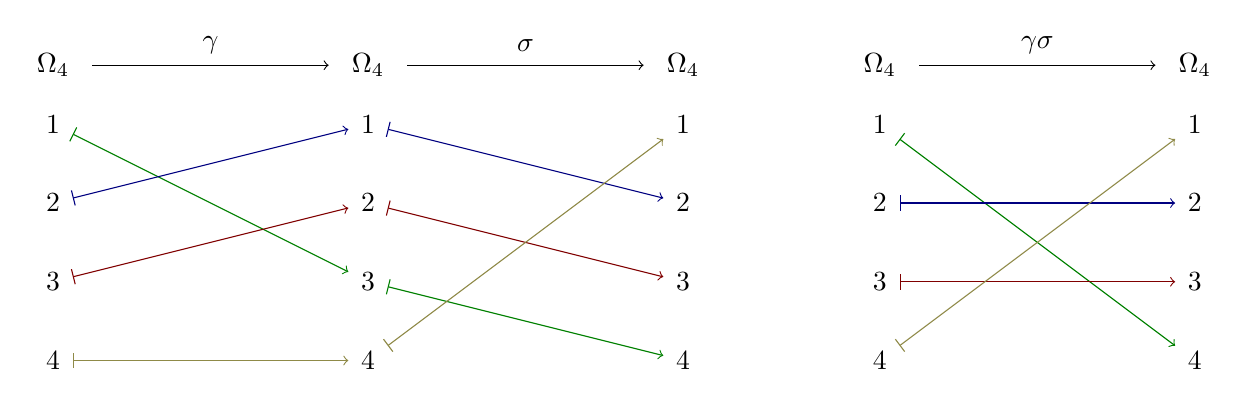
\begin{tikzpicture}[scale=1]
            \begin{scope}[shift={(0, 0)}]
                \foreach \x in {1, 2, 3, 4}
                    \node at (-4, -\x + 4) {$\x$};
                \foreach \x in {1, 2, 3, 4}
                    \node at (0, -\x + 4) {$\x$};
                \foreach \x in {1, 2, 3, 4}
                    \node at (4, -\x + 4) {$\x$};

                \node at (-4, 3.75) {$\Omega_{4}$}; \node at (0, 3.75) {$\Omega_{4}$}; \node at (4, 3.75) {$\Omega_{4}$};
                \draw[->] (-3.5, 3.75) -- (-0.5, 3.75); \node at (-2, 4) {$\gamma$}; \draw[->] (0.5, 3.75) -- (3.5, 3.75); \node at (2, 4) {$\sigma$};

                \draw[|->, green!50!black]  (-3.75, 2.875) -- (-0.25, 1.125);   %  1 -- 3
                \draw[|->, blue!50!black]   (-3.75, 2.0625) -- (-0.25, 2.9375); %  2 -- 1
                \draw[|->, red!50!black]    (-3.75, 1.0625) -- (-0.25, 1.9375); %  3 -- 2
                \draw[|->, yellow!50!black] (-3.75, 0) -- (-0.25, 0);           %  4 -- 4
                \draw[|->, blue!50!black]   (0.25, 2.9375) -- (3.75, 2.0625);   %  1 -- 2
                \draw[|->, red!50!black]    (0.25, 1.9375) -- (3.75, 1.0625);   %  2 -- 3
                \draw[|->, green!50!black]  (0.25, 0.9375) -- (3.75, 0.0625);   %  3 -- 4
                \draw[|->, yellow!50!black] (0.25, 0.1875) -- (3.75, 2.8125);   %  4 -- 1
            \end{scope}
            \begin{scope}[shift={(8.5, 0)}]
                \foreach \x in {1, 2, 3, 4}
                    \node at (-2, -\x + 4) {$\x$};
                \foreach \x in {1, 2, 3, 4}
                    \node at (2, -\x + 4) {$\x$};

                \node at (-2, 3.75) {$\Omega_{4}$}; \node at (2, 3.75) {$\Omega_{4}$}; \draw[->] (-1.5, 3.75) -- (1.5, 3.75); \node at (0, 4) {$\gamma\sigma$};

                \draw[|->, green!50!black]  (-1.75, 2.8125) -- (1.75, 0.1875); %  1 -- 4
                \draw[|->, blue!50!black]   (-1.75, 2) -- (1.75, 2);           %  2 -- 2
                \draw[|->, red!50!black]    (-1.75, 1) -- (1.75, 1);           %  3 -- 3
                \draw[|->, yellow!50!black] (-1.75, 0.1875) -- (1.75, 2.8125); %  4 -- 1
            \end{scope}
        \end{tikzpicture}
        \caption{The diagram of $\gamma\sigma$ as a composition (left) and its simplification (right).}
        \label{fig:gamsigprod2}
    \end{figure}

    This gives us the permutation in two-line form as
    \[
    \gamma\sigma = \begin{pmatrix}
        \textcolor{green!50!black}{1} & \textcolor{blue!50!black}{2} & \textcolor{red!50!black}{3} & \textcolor{yellow!50!black}{4} \\
        \textcolor{green!50!black}{4} & \textcolor{blue!50!black}{2} & \textcolor{red!50!black}{3} & \textcolor{yellow!50!black}{1} \\
    \end{pmatrix},
    \]
    exactly as in the previous method.

    \ulsc{One-line form:} The previous two methods only vary slightly between the left-to-right and right-to-left reading convention. The real intuition for using left-to-right reading convention will begin to become clear in this method.

    The one-line forms of $\gamma$ and $\sigma$ are $\gamma = (1 \q 3 \q 2)$ and $\sigma = (1 \q 2 \q 3 \q 4)$ respectively. Thus, we can initially write $\gamma\sigma$ as
    \[
    \gamma\sigma = (1 \q 3 \q 2)(1 \q 2 \q 3 \q 4).
    \]
    To determine $\gamma\sigma$ as a product of \textit{disjoint} cycles, we appeal to the same strategy: pick any number in the cycles (convention is to start with the smallest number) and write this on the right-hand-side with an open bracket,
    \[
    (1 \q 3 \q 2)(1 \q 2 \q 3 \q 4) = (1
    \]
    The image of $1$ is to be determined. Instead of a composition, we view this just as a product now, so we read the left cycle first and then the right, just as in the two-line form method. Both the permutations \textit{and} the cycles are read left-to-right. Thus, we have that $1 \xmapsto{\gamma} 3$ under $\gamma$, and then $3 \xmapsto{\sigma} 4$ under $\sigma$, so that $1 \xmapsto{\gamma\sigma} 4$. Thus, we write $4$ after the $1$ and then determine the image of $4$,
    \[
    (1 \q 3 \q 2)(1 \q 2 \q 3 \q 4) = (1 \q 4
    \]
    By the same steps, we have that $4 \xmapsto{\gamma} 4$ (since $4$ is a fixed point in $\gamma$ as it hasn't been written) and then $4 \xmapsto{\sigma} 1$ so that $4 \xmapsto{\gamma\sigma} 1$. Since $4$ maps to $1$ which is at the start of the cycle, we close off the open cycle and start again, say with the number $2$,
    \[
    (1 \q 3 \q 2)(1 \q 2 \q 3 \q 4) = (1 \q 4)(2
    \]
    Again by the same steps, we have that $2 \xmapsto{\gamma} 1$ and then $1 \xmapsto{\sigma} 2$ , so that $2 \xmapsto{\gamma\sigma} 2$ so that $2$ is a fixed point under $\gamma\sigma$. Finally, the image of $3$ is to be determined,
    \[
    (1 \q 3 \q 2)(1 \q 2 \q 3 \q 4) = (1 \q 4)(2)(3
    \]
    We have that $3 \xmapsto{\gamma} 2$ and then $2 \xmapsto{\sigma} 3$, so that $3 \xmapsto{\gamma\sigma} 3$ and $3$ is a fixed point,
    \[
    (1 \q 3 \q 2)(1 \q 2 \q 3 \q 4) = (1 \q 4)(2)(3).
    \]
    This exhausts all of the numbers in the cycles, so we are done. Thus, the one-line form of $\gamma\sigma$ is
    \[
    \gamma\sigma = (1 \q 4)(2)(3) = (1 \q 4)
    \]
    since $2$ and $3$ are fixed points under $\gamma\sigma$, and this result agrees with the methods above.
\end{example}

Once again, we remark that using the right-to-left or left-to-right reading convention gives different results, as illustrated by Example~\ref{eg:siggam} and Example~\ref{eg:siggam2}. For this reason, it is incredibly important to be aware of which convention is being used by an author, and which convention one chooses to use themselves.

\begin{example}
    As in Example~\ref{eg:taugamsig}, let $\sigma = (1 \q 2 \q 3 \q 4 \q 5), \gamma = (2 \q 3), \tau = (1 \q 4 \q 5 \q 2)$ be permutations on $\Omega_{5}$, written in one-line form. We shall consider them only in one-line form for this example, and will determine the one-line form of $\tau\gamma\sigma$. First note that
    \[
    \tau\gamma\sigma = (1 \q 4 \q 5 \q 2)(2 \q 3)(1 \q 2 \q 3 \q 4 \q 5).
    \]
    Since we read the permutations left-to-right, the whole method is far more linear than the right-to-left reading convention (in the sense that we \textit{only} read left-to-right). We will start with determining the image of $1$, so we write
    \[
    (1 \q 4 \q 5 \q 2)(2 \q 3)(1 \q 2 \q 3 \q 4 \q 5) = (1
    \]
    To see why this is so linear, observe the following:

    \begin{figure}[h]
        \centering
        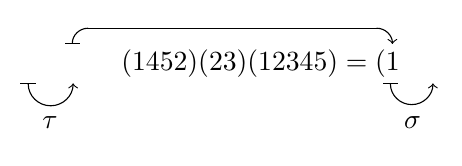
\begin{tikzpicture}
            \node at (0, 0) {$(1 \q 4 \q 5 \q 2)(2 \q 3)(1 \q 2 \q 3 \q 4 \q 5) = (1$};

            \draw[|->] (-2.95, -0.25) arc (-180:0:0.285);
            %\draw[|->] (-2.39, 0.35) -- (1.65, 0.35);
            \draw[|-] (-2.39, 0.25) arc (180:90:0.2);\draw (-2.19, 0.45) -- (1.475, 0.45);\draw[->] (1.475, 0.45) arc (90:0:0.2);
            \draw[|->] (1.65, -0.25) arc (-180:0:0.27);

            \node at (-2.675, -0.75) {$\tau$};\node at (1.93, -0.75) {$\sigma$};
        \end{tikzpicture}
    \end{figure}

    The bottom arrows corresponds to applying a cycle, and the top arrow shows that $4$ is not permuted by the middle cycle. That is, the arrows represent $1 \xmapsto{\tau} 4$ under $\tau$ (the leftmost cycle), then $4$ is fixed by the middle cycle, and then $4 \xmapsto{\sigma} 5$ under $\sigma$ (the rightmost cycle), so that $1 \xmapsto{\tau\gamma\sigma} 5$ and we write a $5$ after the $1$,
    \[
    (1 \q 4 \q 5 \q 2)(2 \q 3)(1 \q 2 \q 3 \q 4 \q 5) = (1 \q 5
    \]
    Again, to exploit the left-to-right reading convention, observe now the image of $5$.

    \begin{figure}[h]
        \centering
        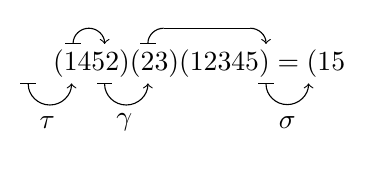
\begin{tikzpicture}
            \node at (0, 0) {$(1 \q 4 \q 5 \q 2)(2 \q 3)(1 \q 2 \q 3 \q 4 \q 5) = (1 \q 5$};

            \draw[|->] (-2.17, -0.25) arc (-180:0:0.275);
            \draw[|->] (-1.2, -0.25) arc (-180:0:0.275);
            \draw[|->] (0.85, -0.25) arc (-180:0:0.27);

            \draw[|-] (-1.6, 0.25) arc (180:90:0.2);\draw[->] (-1.4, 0.45) arc (90:0:0.2);%\draw (-1.8, 0.45) -- (1.475, 0.45);
            \draw[|-] (-0.65, 0.25) arc (180:90:0.2);\draw (-0.45, 0.45) -- (0.65, 0.45);\draw[->] (0.65, 0.45) arc (90:0:0.2);

            \node at (-1.93, -0.75) {$\tau$};\node at (-0.95, -0.75) {$\gamma$};\node at (1.12, -0.75) {$\sigma$};
        \end{tikzpicture}
    \end{figure}

    The bottom arrows represent $5 \xmapsto{\tau} 2 \xmapsto{\gamma} 3 \xmapsto{\sigma} 4$, so that $5 \xmapsto{\tau\gamma\sigma} 4$. Hence, we write $4$ after the $5$,
    \[
    (1 \q 4 \q 5 \q 2)(2 \q 3)(1 \q 2 \q 3 \q 4 \q 5) = (1 \q 5 \q 4
    \]
    To determine the image of $4$ we apply the same process. However, care must be taken when applying the permutation in the rightmost cycle of the left hand side.\newpage

    \begin{figure}[ht]
        \centering
        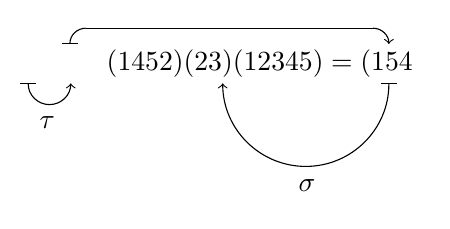
\begin{tikzpicture}
            \node at (0, 0) {$(1 \q 4 \q 5 \q 2)(2 \q 3)(1 \q 2 \q 3 \q 4 \q 5) = (1 \q 5 \q 4$};

            \draw[|->] (-2.94, -0.25) arc (-180:0:0.27);
            \draw[|-] (-2.41, 0.25) arc (180:90:0.2);\draw (-2.21, 0.45) -- (1.44, 0.45);\draw[->] (1.44, 0.45) arc (90:0:0.2);
            \draw[|->] (1.64, -0.25) arc (0:-180:1.055);

            \node at (-2.7, -0.75) {$\tau$};\node at (0.6, -1.55) {$\sigma$};
        \end{tikzpicture}
    \end{figure}

    The only time this `linear' viewpoint fails is at the rightmost element in a cycle, which cycles back to the start of the cycle. This is precisely what happens above in the rightmost cycle of the left hand side. Once again, the bottom arrows corresponds to applying a cycle, and the top arrow shows that $5$ is not permuted by the middle cycle. That is, the arrows correspond to $4 \xmapsto{\tau} 5 \xmapsto{\gamma} 5 \xmapsto{\sigma} 1$, so that $4 \xmapsto{\tau\gamma\sigma} 1$. Since $4$ maps to $1$, we close off the open cycle and open a new cycle with a new number, say $2$,
    \[
    (1 \q 4 \q 5 \q 2)(2 \q 3)(1 \q 2 \q 3 \q 4 \q 5) = (1 \q 5 \q 4)(2
    \]
    Once again, since $2$ is the rightmost element of the first cycle, care must be taken when applying this method.

    \begin{figure}[h]
        \centering
        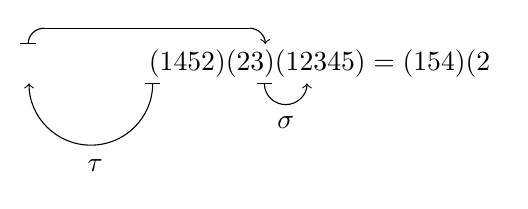
\begin{tikzpicture}
            \node at (0, 0) {$(1 \q 4 \q 5 \q 2)(2 \q 3)(1 \q 2 \q 3 \q 4 \q 5) = (1 \q 5 \q 4)(2$};

            \draw[|->] (-2.12, -0.25) arc (0:-180:0.785);
            \draw[|-] (-3.7, 0.25) arc (180:90:0.2);\draw (-3.5, 0.45) -- (-0.89, 0.45);\draw[->] (-0.89, 0.45) arc (90:0:0.2);
            \draw[|->] (-0.7, -0.25) arc (-180:0:0.27);

            \node at (-2.85, -1.3) {$\tau$};\node at (-0.43, -0.75) {$\sigma$};
        \end{tikzpicture}
    \end{figure}

    The bottom arrows corresponds to applying a cycle, and the top arrow shows that $1$ is not permuted by the middle cycle, so that $2 \xmapsto{\tau} 1 \xmapsto{\gamma} 1 \xmapsto{\sigma} 2$ and thus $2 \xmapsto{\tau\gamma\sigma} 2$. Since $2$ is a fixed point we close off its cycle and open a new one with the remaining number $3$,
    \[
    (1 \q 4 \q 5 \q 2)(2 \q 3)(1 \q 2 \q 3 \q 4 \q 5) = (1 \q 5 \q 4)(2)(3
    \]
    Since $3$ does not appear in the leftmost cycle, we understand $3$ to be fixed by that cycle. This means that $3 \xmapsto{\tau} 3$, and thus we move straight to the next cycle to determine the image of $3$.

    \begin{figure}[h]
        \centering
        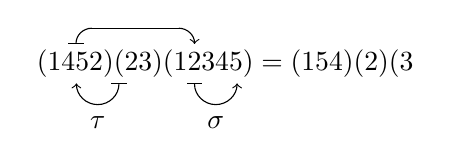
\begin{tikzpicture}
            \node at (0, 0) {$(1 \q 4 \q 5 \q 2)(2 \q 3)(1 \q 2 \q 3 \q 4 \q 5) = (1 \q 5 \q 4)(2)(3$};

            \draw[|->] (-1.35, -0.25) arc (0:-180:0.27);
            \draw[|-] (-1.895, 0.25) arc (180:90:0.2);\draw (-1.695, 0.45) -- (-0.59, 0.45);\draw[->] (-0.59, 0.45) arc (90:0:0.2);
            \draw[|->] (-0.39, -0.25) arc (-180:0:0.27);

            \node at (-1.62, -0.75) {$\tau$};\node at (-0.12, -0.75) {$\sigma$};
        \end{tikzpicture}
    \end{figure}

    The bottom arrows corresponds to applying a cycle, but in this case the top arrow is a reminder of what direction the permutations are being multiplied. Thus $3 \xmapsto{\tau} 3 \xmapsto{\gamma} 2 \xmapsto{\sigma} 3$ so that $3 \xmapsto{\tau\gamma\sigma} 3$ and we close off the cycle,
    \[
    (1 \q 4 \q 5 \q 2)(2 \q 3)(1 \q 2 \q 3 \q 4 \q 5) = (1 \q 5 \q 4)(2)(3).
    \]
    Since this exhausts all of the numbers, we are done. Hence the product $\tau\gamma\sigma$ is given in one-line form as
    \[
    \tau\gamma\sigma = (1 \q 5 \q 4)(2)(3) = (1 \q 5 \q 4).
    \]
    We remark that this is notably different from the composition $\tau\gamma\sigma$ when the right-to-left reading convention is used instead.
\end{example}

There is one more remark to be made. To determine the image of $4$ above we drew the following arrows:

\begin{figure}[ht]
    \centering
    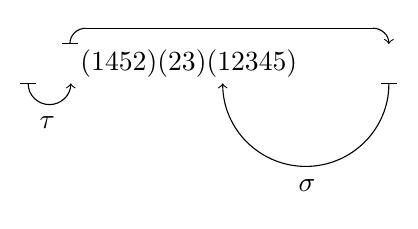
\begin{tikzpicture}
        \node at (0, 0) {$(1 \q 4 \q 5 \q 2)(2 \q 3)(1 \q 2 \q 3 \q 4 \q 5)$};

        \draw[|->] (-2.94+0.9, -0.25) arc (-180:0:0.27);
        \draw[|-] (-2.41+0.9, 0.25) arc (180:90:0.2);\draw (-2.21+0.9, 0.45) -- (1.44+0.9, 0.45);\draw[->] (1.44+0.9, 0.45) arc (90:0:0.2);
        \draw[|->] (1.64+0.9, -0.25) arc (0:-180:1.055);

        \node at (-2.7+0.9, -0.75) {$\tau$};\node at (0.6+0.9, -1.55) {$\sigma$};
    \end{tikzpicture}
\end{figure}

However, recall that the permutations
\[
(1 \q 2 \q 3 \q 4 \q 5) = (5 \q 1 \q 2 \q 3 \q 4) = (4 \q 5 \q 1 \q 2 \q 3) = (3 \q 4 \q 5 \q 1 \q 2) = (2 \q 3 \q 4 \q 5  \q 1)
\]
are all the same, so we can replace $(1 \q 2 \q 3 \q 4 \q 5)$ by any of the equivalent permutations. For example, by picking $(5 \q 1 \q 2 \q 3 \q 4)$ to replace $(1 \q 2 \q 3 \q 4 \q 5)$, the product $\tau\gamma\sigma$ becomes
\[
\tau\gamma\sigma = (1 \q 4 \q 5 \q 2)(2 \q 3)(5 \q 1 \q 2 \q 3 \q 4)
\]
and we can draw the following arrows:

\begin{figure}[h]
    \centering
    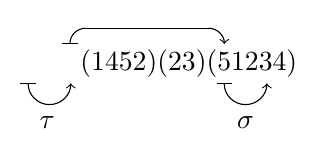
\begin{tikzpicture}
        \node at (0, 0) {$(1 \q 4 \q 5 \q 2)(2 \q 3)(5 \q 1 \q 2 \q 3 \q 4)$};

        \draw[|->] (-2.04, -0.25) arc (-180:0:0.27);
        \draw[|-] (-2.41+0.9, 0.25) arc (180:90:0.2);\draw (-2.21+0.9, 0.45) -- (0.25, 0.45);\draw[->] (0.25, 0.45) arc (90:0:0.2);
        \draw[|->] (0.45, -0.25) arc (-180:0:0.27);

        \node at (-2.7+0.9, -0.75) {$\tau$};\node at (0.72, -0.75) {$\sigma$};
    \end{tikzpicture}
\end{figure}

We see that reading the permutations left-to-right is linear after all! If replacing a cycle with one of its equivalent cycles makes calculations easier, then it is clearly allowed, though one should still endeavour to multiply permutations without having to do such replacements.

%%%%%%%%%%%%%%%%%%%%%%%%%%%%%%%%%%%%%%%%%%
%%%%%%%%%%%%%%%%%%%%%%%%%%%%%%%%%%%%%%%%%%

\subsection{Formal definitions}

The reading conventions explained in the past two sections correspond to whether we `multiply on the right' or `multiply on the left'. To understand what this means, we have to view the operation of multiplication as a map, too. First, we need a set where multiplication makes sense (such as the integers or a group) so consider some set $G$. Typically, multiplication is a binary operation that takes two elements $g, h \in G$ whose image is $g \cdot h$, or more typically just $gh \in G$. This type of multiplication needs two inputs to be evaluated, namely $g$ and $h$. We will define multiplication to be a unary operation that only takes one input, but there is a map corresponding to each element of $G$. We will denote this by $m_{k}$, which will correspond to multiplying the input by $k \in G$. The order of the multiplication depends on whether the map $m_{k}$ defines \textit{right multiplication} or \textit{left multiplication}.

\begin{definition}[(Multiplication)]
    Let $m_{k} \colon G \to G$ be a map from $G$ to $G$ corresponding to the element $k \in G$. Then we say that $m_{k}$ acts by
    \vspace*{-10pt}
    \begin{itemize}[nolistsep]
        \item[--] \textit{right multiplication} (or \textit{multiplication on the right}) if $m_{k}(n) = n \cdot k$;
        \item[--] \textit{left multiplication} (or \textit{multiplication on the left}) if $m_{k}(n) = k \cdot n$.
    \end{itemize}
    \vspace*{-10pt}
    We call the map $m_{k}$ \textit{multiplication by $k$}. It is also common to say that $k$ \textit{acts on the right} (or \textit{left}, respectively).
\end{definition}

For integers, there really is no distinction between left and right multiples since for any two integers $x, y \in \Z$, the product $xy$ and $yx$ are always equal. The distinction becomes important when the binary multiplication is \textit{not} commutative; that is, when $gh \neq hg$ for two general $g, h \in G$. %Example~\ref{eg:siggam} illustrated two such permutations whose product $\gamma\sigma$ was not equal to the product $\sigma\gamma$.

In the cases above, the right-to-left reading convention corresponds to left multiplication, and the left-to-right reading convention corresponds to right multiplication. We will use these names for the conventions from now on, and will see that by doing so the two correspond nicely.

\begin{example}
    Consider multiplication of integers. This is now written formally as $m_{k} \colon \Z \to \Z$, where $m_{k}$ corresponds to multiplication by $k \in \Z$. If $m_{k}$ multiplied on the left, then some examples include
    \[
    m_{2}(5) = 2\cdot 5 = 10, \hspace{20pt} m_{-4}(7) = -4\cdot 7 = -28, \hspace{20pt} m_{9}(4) = 9\cdot 4 = 36.
    \]
    If $m_{k}$ multiplied on the right, then the maps would be evaluated as
    \[
    m_{2}(5) = 5\cdot 2 = 10, \hspace{20pt} m_{-4}(7) = 7\cdot -4 = -28, \hspace{20pt} m_{9}(4) = 4\cdot 9 = 36.
    \]
    Although the numbers have been switched in the product, the products give the same results. This is a well established fact for integers.
\end{example}

\begin{example}
    We can put the product of permutations from Example~\ref{eg:siggam} into a more formal setting now. Let $\sigma = (1 \q 2 \q 3 \q 4)$ and $\gamma = (1 \q 3 \q 2)$ be permutations on $\Omega_{4}$. The map $m_{\sigma}$ corresponds to multiplication by $\sigma$, and the map $m_{\gamma}$ corresponds to multiplication by $\gamma$.

    \ulsc{Left multiplication:} Suppose that $m_{\sigma}$ and $m_{\gamma}$ multiply on the left. Consider the image of $\gamma$ under $m_{\sigma}$. Since the maps multiply on the left, this corresponds to the right-to-left reading convention so that $m_{\sigma}(\gamma) = \sigma\gamma$ and we read $\sigma\gamma$ as $\gamma$ first, followed by $\sigma$. As maps, this product is in fact a composition, so it is helpful to write $\sigma\gamma$ as $\sigma\circ\gamma$ as a reminder that $\gamma$ is evaluated first, followed by $\sigma$. Thus, since $m_{\sigma}$ and $m_{\gamma}$ multiply on the left, we will write
    \[
    m_{\sigma}(\gamma) = \sigma\circ\gamma \textand m_{\gamma}(\sigma) = \gamma\circ\sigma.
    \]
    Now, as we are using the right-to-left reading convention, we have
    \[
    m_{\sigma}(\gamma) = \sigma \circ \gamma = (1 \q 2 \q 3 \q 4)(1 \q 3 \q 2) = (1 \q 4)(2)(3) = (1 \q 4)
    \]
    and also
    \[
    m_{\gamma}(\sigma) = \gamma \circ \sigma = (1 \q 3 \q 2)(1 \q 2 \q 3 \q 4) = (1)(2)(3 \q 4) = (3 \q 4).
    \]
    As we have already discovered, we do not have equality between $\sigma \circ \gamma$ and $\gamma \circ \sigma$.

    \ulsc{Right multiplication:} Suppose that $m_{\sigma}$ and $m_{\gamma}$ multiply on the right. Consider the image of $\gamma$ under $m_{\sigma}$. Since the maps multiply on the right, this corresponds to the left-to-right reading convention so that $m_{\sigma}(\gamma) = \gamma\sigma$ and we read $\gamma\sigma$ as $\gamma$ first, followed by $\sigma$. This can be viewed as a normal product, so it is helpful to write $\gamma\sigma$ as $\gamma\cdot\sigma$ as a reminder that $\gamma$ is evaluated first, followed by $\sigma$. Thus, since $m_{\sigma}$ and $m_{\gamma}$ multiply on the right, we will write
    \[
    m_{\sigma}(\gamma) = \gamma\cdot\sigma \textand m_{\gamma}(\sigma) = \sigma\cdot\gamma.
    \]
    Now, as we are using the left-to-right reading convention, we have
    \[
    m_{\sigma}(\gamma) = \gamma \cdot \sigma = (1 \q 3 \q 2)(1 \q 2 \q 3 \q 4) = (1 \q 4)(2)(3) = (1 \q 4).
    \]
    and also
    \[
    m_{\gamma}(\sigma) = \sigma \cdot \gamma = (1 \q 2 \q 3 \q 4)(1 \q 3 \q 2) = (1)(2)(3 \q 4) = (3 \q 4).
    \]
    Again, we do not have equality between $\sigma \cdot \gamma$ and $\gamma \cdot \sigma$.

    \ulsc{Comparison:} The use of different reading conventions for the left multiplication and right multiplication make the two coincide nicely. That is, we see above that
    \[
    m_{\sigma}(\gamma) = (1 \q 4) \textand m_{\gamma}(\sigma) = (3 \q 4)
    \]
    irrespective of whether we multiply on the left or on the right because we use the correct reading convention for each. We have the equivalence
    \[
    \sigma \circ \gamma = \gamma \cdot \sigma
    \]
    because in both cases $\gamma$ is evaluated first and then $\sigma$, and similarly
    \[
    \gamma \circ \sigma = \sigma \cdot \gamma
    \]
    because in both cases $\sigma$ is evaluated first and then $\gamma$. Exercise~\ref{ex:ch1-ltronly} explores how this changes if one \textit{does not} use the correct reading convention, and shows why it is so important to know which convention is being used at any time.
\end{example}

The understanding of which convention to use is most important when the products are written without a symbol to indicate which convention is being used. Many authors write $\sigma\gamma$ for the product of $\sigma$ and $\gamma$, which gives no indication of which order the permutations are to be multiplied by. Similarly, as above, it is even more uncommon to write a symbol between the explicit permutations. That is, with $\sigma = (1 \q 2 \q 3 \q 4)$ and $\gamma = (1 \q 3 \q 2)$ as above, both $\sigma\circ\gamma$ and $\sigma\cdot\gamma$ are written explicitly as
\[
(1 \q 2 \q 3 \q 4)(1 \q 3 \q 2).
\]
It it always to be taken from context whether one multiplies the above using the left-to-right or the right-to-left reading convention.

%%%%%%%%%%%%%%%%%%%%%%%%%%%%%%%%%%%%%%%%%%
%%%%%%%%%%%%%%%%%%%%%%%%%%%%%%%%%%%%%%%%%%

\subsection{Exercises}

\begin{exercise}\label{ex:ch1-maps}
    Let $f \colon \Omega_{6} \to \Omega_{5}$ be given by
    \[
    f(1) = 2,\q f(2) = 4,\q f(3) = 1,\q f(4) = 3,\q f(5) = 4,\q f(6) = 2.
    \]
    Sketch the diagram of $f$, just as in Figure~\ref{fig:bijmap}. Is $f$ any of injective, surjective, or bijective?
\end{exercise}

\begin{exercise}\label{ex:ch1-fourmethods}
    Let $\sigma = (1 \q 6 \q 4 \q 2 \q 5)$ and $\gamma = (1 \q 5 \q 2 \q 4 \q 6)$ be permutations on $\Omega_{6}$. Write $\sigma$ and $\gamma$ in mapping notation, in two-line form, and in diagrammatic form. Find the product $\sigma\gamma$ using the right-to-left reading convention and then the left-to-right reading convention using all four methods as in Example~\ref{eg:siggam} and Example~\ref{eg:siggam2}.
\end{exercise}

\begin{exercise}\label{ex:ch1-notpermutations}
    Determine which of the following are not permutations:
    \[
    \sigma_{1} = \begin{pmatrix}
        1 & 2 & 3 & 4 & 5 \\
        3 & 2 & 1 & 5 & 4 \\
    \end{pmatrix},\, \sigma_{2} = \begin{pmatrix}
        1 & 2 & 3 & 4 & 5 \\
        5 & 1 & 4 & 2 & 4 \\
    \end{pmatrix},\, \sigma_{3} = \begin{pmatrix}
        1 & 2 & 3 & 4 & 5 \\
        1 & 2 & 3 & 4 & 5 \\
    \end{pmatrix},\, \sigma_{4} = \begin{pmatrix}
        1 & 2 & 3 & 4 & 5 \\
        4 & 1 & 7 & 5 & 3 \\
    \end{pmatrix}.
    \]
    Of those that \textit{are} permutations, write them in one-line form and in diagrammatic form.
\end{exercise}

\begin{exercise}\label{ex:ch1-frontcover}
    Determine the one-line form and two-line form of the permutation given in diagrammatic form on the front cover.
\end{exercise}

\begin{exercise}\label{ex:ch1-powers}
    Let $\sigma = (1 \q 6 \q 4 \q 2 \q 5)$ and $\gamma = (1 \q 5 \q 2 \q 4 \q 6)$ be permutations on $\Omega_{6}$. We can write $\sigma^{2}$ short for $\sigma\sigma$, and by extending this we can write $\sigma^{n}$ for $n$ copies of $\sigma$ all multiplied together. Compute the powers of $\sigma$ and of $\gamma$ up to $n = 6$ (that is, compute $\sigma^{i}$ and $\gamma^{i}$ for $i \in \{2, 3, 4, 5, 6\}$). Is there a relationship between the powers of $\sigma$ and the powers of $\gamma$?
\end{exercise}

\begin{exercise}\label{ex:ch1-rtl&ltr}
    Compute the following products using the right-to-left reading convention and then the left-to-right reading convention.
    \vspace*{-10pt}
    \begin{itemize}[nolistsep]
        \item[(a)] \q$(2 \q 4 \q 6 \q 1 \q 3 \q 5)(2 \q 1)(4 \q 3)(6 \q 5)(2 \q 6 \q 3)(4 \q 1 \q 5)$;
        \item[(b)] \q$(1 \q 2 \q 3)(2 \q 3 \q 4)(3 \q 4 \q 5)(3 \q 2 \q 1)(4 \q 3 \q 2)(5 \q 4 \q 3)$;
        \item[(c)] \q$(1 \q 2 \q 3 \q 4)(3 \q 6 \q 5 \q 2 \q 1 \q 4)(1 \q 4 \q 3 \q 2)$;
        \item[(d)] \q$(1 \q 2)(1 \q 3)(1 \q 4)(1 \q 5)(1 \q 6)(1 \q 7)(1 \q 8)$;
    \end{itemize}
\end{exercise}

\begin{exercise}\label{ex:ch1-ltronly}
    Let $\sigma = (1 \q 3 \q 2 \q 4)$, $\gamma = (2 \q 3 \q 4)$, and $\tau = (1 \q 4 \q 5)$. Consider, for this exercise only, that multiplying on the left and multiplying on the right both use the left-to-right reading convention. Compute each of
    \[
    m_{\sigma}(\gamma),\q m_{\sigma}(\tau),\q m_{\sigma}(\gamma\cdot\tau),\q m_{\sigma}(\tau\cdot\gamma),\q m_{\sigma}(\gamma^{2}),\q m_{\sigma}(\tau^{2})
    \]
    given that
    \vspace*{-10pt}
    \begin{itemize}[nolistsep]
        \item[(a)] $m$ multiplies on the left;
        \item[(b)] $m$ multiplies on the right.
    \end{itemize}
\end{exercise}

\begin{exercise}\label{ex:ch1-omegainfty}
    Let $\sigma = (2 \q 4 \q 6)$ be a permutation in one-line form. Determine on which of the following sets this permutation is defined:
    \[
    \Omega_{1},\quad \Omega_{4},\quad \Omega_{6},\quad \Omega_{10},\quad \Omega_{10^{100}},\quad \Omega_{\infty}.
    \]
    Here we identify $\Omega_{\infty}$ with the naturals numbers $\N = \{1, 2, 3, \ldots\}$. That is, we define $\Omega_{\infty} = \N$.
\end{exercise}

\begin{exercise}\label{ex:ch1-reduced_two-line_form}
    This is an exercise in using the reduced two-line form. Recall that in this notation, the number in the \(i^{\text{th}}\) position is the image of \(i\) under the permutation. For example, the permutation \((2 \q 1 \q 3)\) is understood as
    \[
    1 \mapsto 2,\qquad 2 \mapsto 1,\textand 3 \mapsto 3.
    \]
    Compute the following products using the right-to-left reading convention and then the left-to-right reading convention.
    \vspace*{-10pt}
    \begin{itemize}[nolistsep]
        \item[(a)] \q\((1 \q 3 \q 2 \q 4)(4 \q 2 \q 1 \q 3)(2 \q 1 \q 3 \q 4)\);
        \item[(b)] \q\((2 \q 3 \q 4 \q 1)(3 \q 4 \q 1 \q 2)(4 \q 1 \q 2 \q 3)\);
    \end{itemize}
\end{exercise}